\section{Versuchsdurchführung}
\subsection{Versuchsaufbau}
\subsubsection{Hardware}
Der Versuchsaufbau besteht aus zwei Platinen:
\begin{itemize}
    \item \textbf{Transistorplatine:} Diese beinhaltet die Leistungstransistoren und die Temperatursensoren.
    \item \textbf{Controllerplatine:} Diese dient zur Messerfassung mittels eines PSoC.
\end{itemize}
\begin{figure}[H]
    \centering
    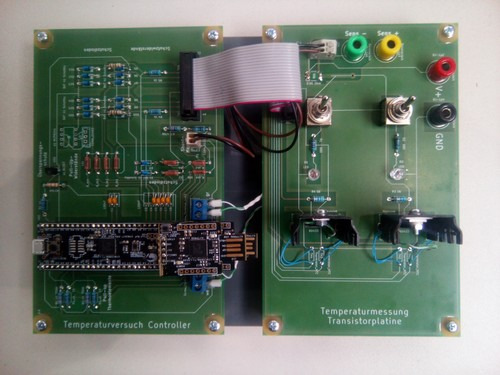
\includegraphics[width=0.7\textwidth]{images/versuchsschaltung.jpeg}
    \caption{Übersicht über die gesamte Versuchsschaltung mit Controllerplatine links
        und Transistorplatine rechts.}
    \label{fig:versuchsschaltung}
\end{figure}
Auf der Transistorplatine sind zwei Leistungstransistoren zum Ausmessen aufgebaut. Diese sind mit einem Kühlkörper verbunden, auf dem sich die Temperatursensoren befinden. Der Unterschied zwischen den beiden Transistoren besteht darin, dass einer mit einer zusätzlichen Keramikscheibe zur thermischen Isolation ausgestattet ist. Die Controllerplatine beinhaltet den PSoC-Mikrocontroller, der die Messwerte der Temperatursensoren ausliest und an den PC weiterleitet. 

Zum Aufheizen des Transistors wird ein Labornetzgerät verwendet, dessen Ausgangsstrom auf \SI{1.5}{\ampere} begrenzt ist. Um die Kollektor-Emitter-Spannung und den Strom in der Software zu überwachen, werden zwei Digitalmultimeter verwendet. Diese kommunizieren über eine serielle Schnittstelle mit dem PC.

\subsubsection{Software}
Zur Visualisierung der Messergebnisse wird eine Python-Software verwendet, welche die Daten vom PSoC-Mikrocontroller über eine serielle Schnittstelle empfängt und in Echtzeit darstellt. 
Es gibt die Möglichkeit, zwischen den beiden Transistoren zu wählen. Je nach ausgewähltem Transistor können bis zu drei verschiedene Temperatursensoren dargestellt werden. Um eine Messung zu starten, muss zunächst die Messdauer angegeben und anschließend die Verbindung zur Platine überprüft werden. 
Nach Ende der Messung werden die Daten in einer CSV-Datei und als Bild gespeichert. 

\subsection{Durchführung}
Es gibt insgesamt zwei Messdurchläufe, jeweils einen pro Transistor. Pro Transistor wird für eine Zeitdauer von $10\tau$, d.h. \SI{1200}{\second}, gemessen. Hierbei werden für jeweils \SI{600}{\second} die Aufheizphase und die Abkühlphase erfasst. Um eine korrekte Messung zu erhalten, muss eine Basislinie erfasst werden, indem der jeweilige Schalter erst ca. \SI{15}{\second} nach Start der Messung umgelegt wird.